% ****** Start of file apssamp.tex ******
%
%   This file is part of the APS files in the REVTeX 4.1 distribution.
%   Version 4.1r of REVTeX, August 2010
%
%   Copyright (c) 2009, 2010 The American Physical Society.
%
%   See the REVTeX 4 README file for restrictions and more information.
%
% TeX'ing this file requires that you have AMS-LaTeX 2.0 installed
% as well as the rest of the prerequisites for REVTeX 4.1
%
% See the REVTeX 4 README file
% It also requires running BibTeX. The commands are as follows:
%
%  1)  latex apssamp.tex
%  2)  bibtex apssamp
%  3)  latex apssamp.tex
%  4)  latex apssamp.tex
%
\documentclass[%
 reprint,
%superscriptaddress,
%groupedaddress,
%unsortedaddress,
%runinaddress,
%frontmatterverbose, 
%preprint,
%showpacs,preprintnumbers,
%nofootinbib,
%nobibnotes,
%bibnotes,
 amsmath,amssymb,
 aps,
%pra,
%prb,
%rmp,
%prstab,
%prstper,
%floatfix,
showkeys,
letter,
12pts
]{revtex4-1}

\usepackage{graphicx}% Include figure files
\usepackage{dcolumn}% Align table columns on decimal point
\usepackage{bm}% bold math
%\usepackage{hyperref}% add hypertext capabilities
%\usepackage[mathlines]{lineno}% Enable numbering of text and display math
%\linenumbers\relax % Commence numbering lines

%\usepackage[showframe,%Uncomment any one of the following lines to test 
%%scale=0.7, marginratio={1:1, 2:3}, ignoreall,% default settings
%%text={7in,10in},centering,
%%margin=1.5in,
%%total={6.5in,8.75in}, top=1.2in, left=0.9in, includefoot,
%%height=10in,a5paper,hmargin={3cm,0.8in},
%]{geometry}

%Paquetes que yo agregué
\usepackage[utf8]{inputenc}
\usepackage[spanish]{babel}
%\usepackage{cite}
\usepackage[sort&compress]{natbib}
\bibliographystyle{apalike}


\begin{document}

\preprint{APS/123-QED}

\title{Filogenia de bacterias pertenecientes a la familia \textit{Enterobacteriaceae} por medio de electroforesis SDS-PAGE en Gel de Policrilamida Vertical}% Force line breaks with \\
\thanks{Laboratorio de Biología Molecular - Artículo 1}%

\author{Angie Ramos}
% \altaffiliation[Also at ]{Physics Department, XYZ University.}%Lines break automatically or can be forced with \\
\author{Daniel Molano}%
 %\email{Second.Author@institution.edu}
\author{Elkin Alvis}
% \altaffiliation[Also at ]{Physics Department, XYZ University.}%Lines break automatically or can be forced with \\
\author{Sof\'ia Ardila}
% \altaffiliation[Also at ]{Physics Department, XYZ University.}%Lines break automatically or can be forced with \\

\affiliation{ Universidad de los Andes\\ 
 Bogotá D.C. - Colombia}%


\date[Fecha: ]{\today}% It is always \today, today,
             %  but any date may be explicitly specified

\begin{abstract} %DONE!!
	La proteómica es el estudio sistemático de las proteínas presentes en el genoma de un individuo, posibilitando la identificación, caracterización y función del proteoma global. En esencia, la proteómica se ha presentado como una herramienta que brinda información tanto biológica como evolutiva del organismo o especie. Para el estudio de la misma, la técnica empleada es la electroforesis de poliacrilamida (SDS-PAGE), que consiste en la separación en función de la masa molecular que presenta la proteína, confiriendo unificación de cargas. En este estudio, se emplearon distintas cepas bacterianas pertenecientes a la familia \textit{Enterobacteriaceae}. El objetivo consistió en la determinación de las discrepancias y homologías de los proteomas presentes en  las bacterias \textit{Escherichia coli W, Escherichia coli K12, Escherichia coli C600, Yersinia enterocolitica, Salmonella typhi y Proteus spp} empleando electroforesis en gel de poliacrilamida vertical. Para ello, se realizó una extracción proteica de las seis bacterias, y cada una de las muestras fue expuesta a un corrimiento en gel utilizando electroforesis denaturante SDS-PAGE, seguido de una tinción con Azul de Coomassie. Posteriormente, se realizó un análisis proteico relacionando evolutivamente, por medio de la construcción de fenogramas con los métodos UPGMA y NJ. Los perfiles proteicos obtenidos demuestran una cercanía evolutiva entre las cepas de \textit{E. coli} analizadas y \textit{Proteus spp}.
	 
\end{abstract}

\keywords{\textit{Enterobacteriaceae}, Electroforesis en Gel Vertical, Gel de Poliacrilamida, SDS-PAGE, Tinción, Azul de Coomasie, Fenograma}%Use showkeys class option if keyword
                              %display desired
\maketitle

%\tableofcontents

\section{\label{sec:Intro}Introducción}
	La proteómica es una técnica empleada para el estudio de las proteínas de un individuo \cite{intro1}. En la última década, la proteómica microbiana ha generado avances que ofrecen la  posibilidad de comprender totalmente los sistemas microbianos, la evolución y el mecanismo patogénico\cite{intro1}. Gracias a esta técnica ha sido posible verificar los resultados de forma minuciosa, diversas muestras de interés en áreas como biología molecular, bioinformática, bioquímica entre otras, las cuales han evaluado y desarrollado técnicas que permiten el procesamiento y análisis de la información adquirida. En esencia, la proximidad filogenética y biológica es directamente proporcional al número de proteínas compartidas entre diversos organismos, es decir, el número de compatibilidad de bandas en el gel de electroforesis.
	
	Uno de los instrumentos más utilizados para analizar y separar el proteoma es la electroforesis en geles de poliacrilamida, la cual contiene dodecil-sulfato sódico (SDS), que habilita la separación proteica en función de su peso molecular. La técnica SDS-PAGE combina, generalmente, la separación del proteoma teniendo en cuenta su punso isoelectrico y, adicionalmente, la separación de acuerdo a  esas propiedades isoeléctricas. Su tamaño permite el aislamiento en el gel discontinuo, por lo que ésta técnica permite, analizar de forma individual la muestra.
	
	En este estudio se utilizaron  bacterias pertenecientes a la familia Enterobacteriaceae, las cuales, forman un conjunto diverso de microorganismos, donde generalmente se encuentran microorganismos patógenos de plantas, animales y vegetales, entre otros. Los patógenos más destacados son diversos serotipos de las bacterias Escherichia coli, Salmonella spp, Yersinia enterocolitica, éstos microorganismos son agentes causales de ETAs especialmente (Enfermedades transmitidas por alimentos). Se caraterizan por ser anaerobios facultativos, gram negativos, catalasa positiva y oxidasa negativa\cite{intro2}. Sin embargo, muchas de estas características son determinadas utilizando la microbiología clásica, que requiere más tiempo para la lectura y análisis de resultados. Por ello, surge la necesidad de emplear nuevas estrategias que permitan determinar características o muestras de interés en el menor tiempo posible, con la garantía de obtener resultados confiables.
	
	El objetivo de este estudio  es realizar una comparación de los perfiles protéicos de las cepas bacterianas \textit{Escherichia coli C600, E. coli K12, E.coli W, Proteus spp, Salmonella typhi} y \textit{Yersinia enterocolitica}. De forma que evalue las similitudes y discrepancias  por medio de programas como PAUP, NJ y UPGMA, los cuales brindan medidas de similitud entre estas por medio de fenogramas.
	

\section{\label{sec:MyM}Materiales y Métodos} %Final Editing
	Para este estudio se utilizaron proteínas bacterianas de \textit{E. coli W, E. coli K12, E. coli C600, Yersinia enterocolitica, Salmonella typhi y Proteus spp},  todas pertenecientes a la familia \textit{Enterobacteriaceae}; a continuación se enuncian los pasos seguidos para determinar su relación filogenética.
	Primero se realizó la extracción de proteínas de las células correspondientes, luego se realizó una electroforesis SDS-PAGE en gel de poliacrilamida vertical y se procedió a teñir con azul de Coomasie. Se analizó el patrón de bandas obtenido utilizando la herramienta computacional \textit{PAUP} obteniendo finalmente los fenogramas correspondientes, con los cuales se pudo determinar la relación filogenética entre las bacterias estudiadas. Las siguientes secciones describen en detalle cada uno de los procedimientos enunciados.
	
	\subsection{\label{sec:ExtraMet}Extracción de Proteínas Bacterianas}\cite{guia}
		El primer paso para determinar las relaciones filogenéticas de las bacterias en estudio es extraer las proteínas de las células.
		Se comienza dejando las bacterias en crecimiento ON (Over Night) en caldo LB con una agitación de 250$rpm$. Una vez terminado el crecimiento, se procede a medir con una micropipeta 1$ml$ de cada uno de los cultivos y se colocan en \textit{eppendorfs} individuales. Se centrifugan las muestras a 13$Mrpm$ durante 5 minutos; seguidamente, se descarta 800$\mu l$ de la solución en hipoclorito diluido. Los 200$\mu l$ restantes fueron se resuspenden con vórtex. Se añade, a continuación, 100$\mu l$ de \textit{buffer} (contiene SDS), correspondientes a $\frac{1}{2}$ del volumen de cada una de las soluciones con las muestras en los eppendorfs. Luego éstos se pusieron en una plancha de calentamiento durante 5 minutos a 100$^{\circ}C$. Posteriormente se centrifugaron a 13$Mrpm$ por 5 minutos, y finalmente, se extraen de cada una de las muestras el sobrenadante donde se encuentran las proteínas de interés.
		
	%	Es importante mencionar que el \textit{buffer} utilizado contenía detergente SDS (Sodium bla bla) que adiciona la carga negativa a la muestra.También es pertinente resaltar que la presencia del glicerol fue fundamental para evitar la formación de cristales y el congelamiento que podían alterar a muestra, de igual muestra, el azul de bromofenol fue relevante al permitir visualizar el frente de corrido. 
			
	\subsection{\label{sec:ElectroMet}Electroforesis en geles de Poliacrilamida}\cite{guia}
		Posterior a la extracción de proteínas se procede a realizar la electroforesis en geles de poliacrilamida vertical. 
		
		Se comienza preparando los geles. El primero a preparar es el gel de separación; se prepara este gel a una concentración del 10\% debido a que las proteínas en cuestión se encuentran en el rango de 16-70$KDa$. El primer paso es mezclar en un beaker 2$ml$ de solución de poliacrilamida, 1.25$ml$ de una solución con pH 8.8 y 1.75$ml$ de $H_2O$. A continuación se adicionan simultáneamente 50$\mu l$ de persulfato de amonio al 10\% y 8$\mu l$ de TEMED. Inmediatamente se vierte dentro de la cámara del montaje y se deja polimerizar unos 45 minutos. Para el gel de agrupamiento, se comienza mezclando en un beaker 325$\mu l$ de poliacrilamida, 625$\mu l$ de una solución con pH 6.8 y 1525$\mu l$ de $H_2O$. Luego se adiciona simultáneamente 25$\mu l$ de persulfato de amonio al 10\% y 5$\mu l$ de TEMED, se agita bien y se vierte en la cavidad del montaje, se ponen los peines para crear los pozos y se deja polimerizar por 15 minutos. Transcurrido este tiempo se pueden retirar los peines y proceder con el montaje de la cámara de electroforesis. El montaje debe verse similar al mostrado en la figura \ref{Imagen: SDS-PAGE}.
		
		\begin{figure}[h]
		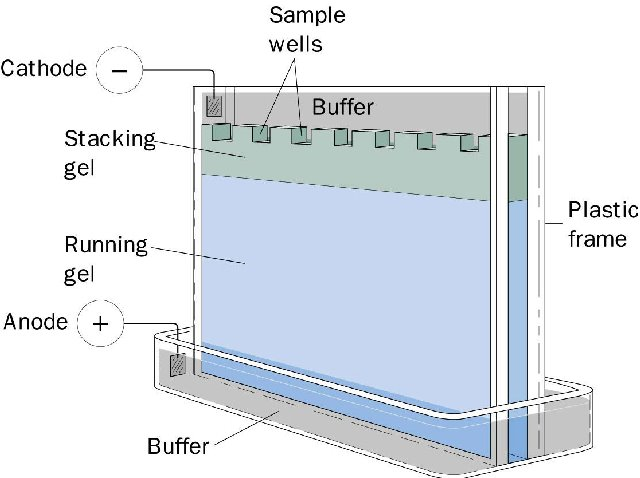
\includegraphics[width=0.4\textwidth]{SDS-PAGE.jpg}
		\caption{SDS-PAGE. La imagen muestra el montaje justo antes de realizar a siembra de las muestras.}
		\label{Imagen: SDS-PAGE}
		\end{figure} 

		Para realizar el montaje de la cámara electroforética, se asegura el o los pares de geles en el interior de esta. Se llena la cámara interna con \textit{buffer} de electroforesis 1X hasta que cubra los pozos y vierta el resto del \textit{buffer} en la cámara externa. Se continúa sembrando 8$\mu l$ de cada una de las muestras. Terminado el sembrado, se cierra apropiadamente la cámara y se programa el corrido de electroforesis a 150$V$ y 90 minutos. Una vez terminado el corrido se procede a fijarlo. Para esto se prepara una solución de fijado, que se compone de 50\% de etanol, 10\% de ácido acético y 40\% de $dH_2O$. Esta solución se vierte en las cubetas del kit y a continuación se desmonta el gel de la cámara. Primero se apaga y desconecta la fuente de poder, se retira el montaje de los vidrios y se separa con cuidado el gel de estos. Se remueve y se descarta el gel de agrupamiento y se hace un pequeño corte en alguna esquina para identificar la ubicación del primer carril del gel. A paso seguido se deposita el gel en la cubeta con la solución de fijado y se guarda la el gel a 4$^{\circ}C$ por 8 días.

		%Nota: Cabe resaltar que en el gel se siembran proteínas de 2 bacterias más: bla1 y bla2. Estas fueron suministradas por el docente al momento de la siembra.
		
	\subsection{\label{sec:TinMet}Tinción con Azul de Coomasie}\cite{guia}
		Una vez el gel esté fijado, se tiñe con Azul de Coomasie para ver el patrón de bandeo.
		
		Se prepara la solución de tinción mezclando 50\% de metanol, 10\% de ácido acético, 40\% de $dH_2O$ y Coomasie al 0.05\%. Se Retira la solución de fijación de la cubeta, cuidando que el gel no quede con pliegues, se agrega la solución de tinción y se deja en agitación continua a aproximadamente 60$rpm$ y 37$^{\circ}C$ durante 45 minutos. Transcurrido el tiempo, se descarta la solución de tinción y se hace un lavado $dH_2O$. Seguido de esto, se agrega la solución de destinción previamente preparada así: 50\% de metanol, 10\% de ácido acético y 40\% de $dH_2O$. La cubeta con el gel en la solución de destinción, se deja en agitación constante a 50$rpm$ y 37$^{\circ}C$ hasta que se obtiene la intensidad de las bandas deseada.
		
		Obtenido el bandeo deseado, se retira el gel de la solución de destinción y se pone a secar en papel celofán en frío toda una noche.
		
	\subsection{\label{sec:Fen}Construcción del fenograma}\cite{metodos}
		Una vez seco el gel, se procede al reconocimiento y conteo de bandas para su análisis, y se utiliza \textit{PAUP\ 4 Beta} y \textit{FigTree v1.4.2} para la construcción, modificación y análisis de los fenogramas.
		
		Al tener identificadas las bandas presentes para cada uno de los organismo se puede hacer una matriz binaria, unos y ceros, para representar ausencia $\left(0\right)$ o presencia $\left(1\right)$ de cada proteína en cada celda del gel. Construida la matriz, se redacta un archivo .nex en el que se incluye el número de individuos, un nombre provisional para cada uno, por ejemplo Individuo 1, el número de celdas de la matriz y finalmente la matriz, cuidando que cada bacteria ocupe una fila. Se procede a cargar los datos a \textit{PAUP} a través de este archivo. Realizada la carga de los datos, se ejecuta el comando NJ; este habilita la creación de un árbol filogenético por medio del análisis algorítmico de \textbf{Neighbor Joining} el cual “es un método puramente algorítmico, representando una aproximación heurística para encontrar el árbol de evolución mínima más corto” \cite{metodos}, es decir, el que implique menos pasos. Seguidamente, se ejecuta el comando UPGMA crea un árbol filogenético utilizando el análisis \textbf{Unweighted Pair Group Method Using Average Linkage} el cual “se puede concebir como un método heurístico para encontrar la topología ultramarina---todas las ojas equidistantes a la raíz---de mínimos cuadrados para una matriz de distancias pareadas” \cite{metodos}. Obtenidos los árboles podemos visualizarlos y editarlos en \textit{FigTree}. Después de realizar los cambios pertinentes y editar el árbol de manera que fuese sencilla su lectura, se guardan las imágenes para su posterior análisis.	
	
\section{\label{sec:Resul}Resultados} %
	\subsection{El gel y patrón de bandeo}
		Al terminar el proceso de tinción y destinción con azul de Coomasie descrito arriba, se obtienen los primeros resultados visibles: un patrón de bandeo en el gel de poliacrilamida. Dicho patrón comprueba la presencia de proteínas en el gel así como también que los procedimientos anteriores fueron desarrollados con éxito. A continuación se muestra una imagen del gel húmedo ---figura \ref{Imagen:gelI}--- justo antes de iniciar el proceso de secado; y una segunda figura que muestra el gel en su estado final ---figura \ref{Imagen:gelII}.
		
		\begin{figure}
		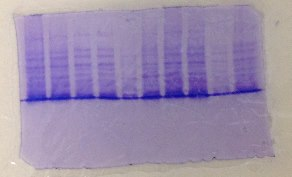
\includegraphics[width=0.47\textwidth]{foto1.jpg}
		\caption{\textbf{Fotografía del gel húmedo}, justo después de terminar el proceso de destinción y siendo preparado para su secado. Se observa el patrón de bandeo con facilidad.}
		\label{Imagen:gelI}
		\end{figure} 
		
		\begin{figure}
		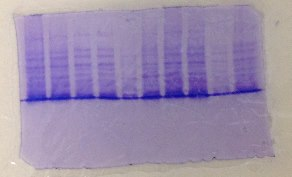
\includegraphics[width=0.5\textwidth]{foto1.jpg}
		\caption{\textbf{Fotografía del gel seco}. Se observa con mayor claridad y nitidez las bandas de cada una de las muestras.}
		\label{Imagen:gelII}
		\end{figure} 
	
	\subsection{La matriz y los árboles}
		La obtención de bandas claramente definidas en el gel, permitió la elaboración de la matriz binaria y su correcto análisis.
		\begin{table}[h!]
			\centering
			\large
			\caption{\textbf{Matriz Binaria} obtenida a partir de la lectura de las bandas en el gel seco.}
			\label{tabla:Matriz}
			\begin{tabular}{|l||l|l|l|l|l|l|l|l|l|l|l|}
			\hline		
			\textbf{Banda} & \textbf{1} & \textbf{2} & \textbf{3} & \textbf{4} & \textbf{5} & \textbf{6} & \textbf{7} & \textbf{8} & \textbf{9} & \textbf{10} & \textbf{11}\\ \hline \hline
			\textbf{\textit{E. Coli C600}} & 1 & 1 & 1 & 1 & 1 & 1 & 1 & 1 & 1 & 0 & 1\\ \hline
			\textbf{\textit{E. Coli K12}}  & 1 & 1 & 1 & 1 & 1 & 1 & 1 & 1 & 1 & 0 & 1\\ \hline
			\textbf{\textit{E. Coli W}}    & 1 & 0 & 1 & 1 & 1 & 1 & 1 & 1 & 1 & 0 & 1\\ \hline
			\textbf{\textit{Proteus}}      & 1 & 0 & 1 & 1 & 1 & 1 & 1 & 1 & 1 & 0 & 1\\ \hline
			\textbf{\textit{Salmonela}}    & 0 & 0 & 1 & 1 & 1 & 0 & 0 & 1 & 0 & 1 & 1\\ \hline
			\textbf{\textit{Yersenia}}     & 1 & 0 & 1 & 1 & 1 & 1 & 0 & 1 & 1 & 1 & 1\\ \hline
			\end{tabular}
		\end{table}	
		
		Luego de completar con los campos requeridos en el archivo .nex, y cargarlo correctamente al programa, se pudo correr los dos diferentes algoritmos y visualizar sus resultados. Los esquemas siguientes representan los resultados obtenidos en su forma gráfica, siendo la figura \ref{Grafica:Nj} el resultado arrojado por NJ y la figura \ref{Grafica:UPGMA} el que se logró con UPGMA.
		
		\begin{figure}[h!]
		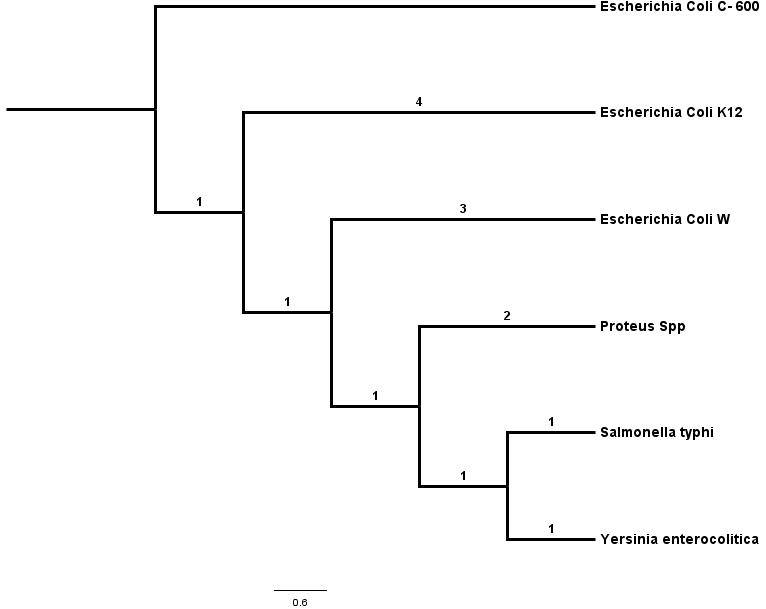
\includegraphics[width=0.5\textwidth]{arbolNJ.jpg}
		\caption{\textbf{Árbol NJ:} Fenograma obtenido luego de correr el algoritmo NJ y hacer algunas ediciones para su mejor visualización y lectura.}
		\label{Grafica:Nj}	
		\end{figure}
	
		\begin{figure}[h!]
		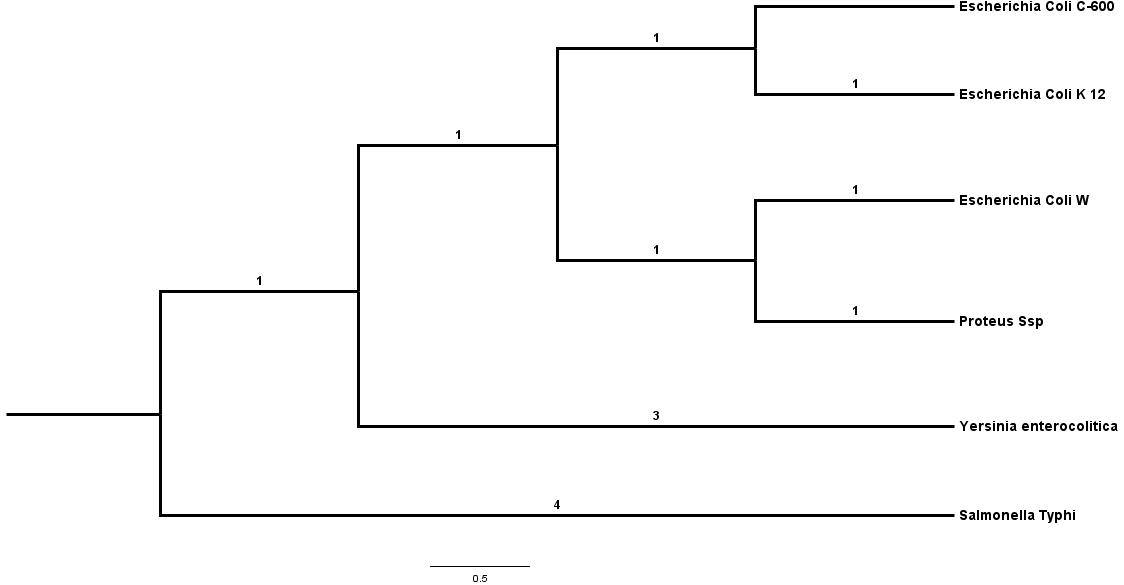
\includegraphics[width=0.5\textwidth]{arbolUPGMA.jpg}
		\caption{\textbf{Árbol UPGMA:} Fenograma obtenido luego de correo el algoritmo UPGMA y hacer algunas ediciones para su mejor visualización y lectura.}
		\label{Grafica:UPGMA}
		\end{figure}	
		
		Estos son los resultados finales y esperados, los cuales pueden ser analizados de manera directa, clara y concisa.

\section{\label{sec:Dis}Discusión de Resultados}
	Los esquemas obtenidos muestran las relaciones filogenéticas de los organismos analizados. Se puede concluir del la figura \ref{Grafica:UPGMA}, que \textit{E. coli C600} es muy cercana a \textit{E. coli K12}. De la misma manera se observa una cercanía estrecha entre \textit{E. coli W} con \textit{Proteus spp}. Estas cuatro sepas muestran también una cercanía entre sí, aunque menor a la mencionada anteriormente. Finalmente, se puede anotar que la más cercana a las cuatro primeras es \textit{Yersenia enterocolitica} y la más lejana del grupo es \textit{Salmonela typhi}.
	
	Con los resultados obtenidos se confirmó la relación filogenéticas existentes entre las distintas cepas analizadas. De la misma forma, y al comparar con la literatura, se concluyó que las relaciones de cercanía obtenidas son aproximadamente correctas.
	
	Sobre el patrón obtenido del gel, se puede decir que todo el procedimiento se realizó de manera correcta, ya que la obtención del bandeo así como el de las relaciones filogenéticas fueron acertadas.
	
	Los posibles errores experimentales pueden atribuirse a inexperiencia en la ejecución de los experimentos, en especial el proceso de tinción y destición, ya que esto puedo afectar la cantidad y calidad de las bandas observadas. De igual manera, la sensibilidad de lectura de cada persona afecta la obtención de la matriz; entre más bandas se identifiquen más preciso y detallado será las aproximaciones obtenidas. Otra fuente de error es la incertidumbre de los instrumentos, aunque en esta ocasión fueron pocas mediciones, esto pudo afectar la resolución de las bandas observadas.
	
	Teniendo en cuenta todo lo mencionado anteriormente, se afirma que el objetivo de la práctica se cumplió a satisfacción, determinando con gran similitud la filogenias de las cepas bacterianas dadas.	
	
	
	

\bibliographystyle{apalike}
\bibliography{proteinasBib}
\end{document}
%
% ****** End of file apssamp.tex ******
